%% Running Head
\begin{flushright}
  {\small\textsf{\textbf{MỤC 3.9}\quad Tốc độ liên thuộc}\qquad {\large\textbf{247}}}
\end{flushright}
\vspace{2pt}

%% Applied Project Box (Full Width)
\begin{tcolorbox}[
  colback=lightgreenbg,
  colframe=lightgreenbg,
  arc=0mm,
  boxrule=0pt,
  left=6pt, right=8pt, top=4pt, bottom=6pt
]
  %% Title Banner
  \begin{center}
    \begin{tikzpicture}[baseline=(T.base)]
      \foreach \y in {-4pt, -2pt, 0pt, 2pt, 4pt} {
        \draw[stewartgreen, thin] (-6.5,\y) -- (-4.3,\y);
        \draw[stewartgreen, thin] (4.3,\y) -- (6.5,\y);
      }
      \node[inner sep=2pt] (T) at (0,0) {\large\textsf{\textbf{\color{stewartgreen}DỰ ÁN ỨNG DỤNG}}\quad {\normalsize\textbf{\color{stewartgreen}KIỂM SOÁT SỰ MẤT HỒNG CẦU TRONG PHẪU THUẬT}}};
    \end{tikzpicture}
  \end{center}
  \vspace{-4pt}

  %% Content inside box
  \begin{minipage}[t]{0.26\textwidth}
    \vspace{0pt}
    \begin{minipage}{7pt}
      \rotatebox{90}{\tiny\color{gray}Kent Weakley / Shutterstock.com}
    \end{minipage}%
    \hfill
    \begin{minipage}{0.9\textwidth}
      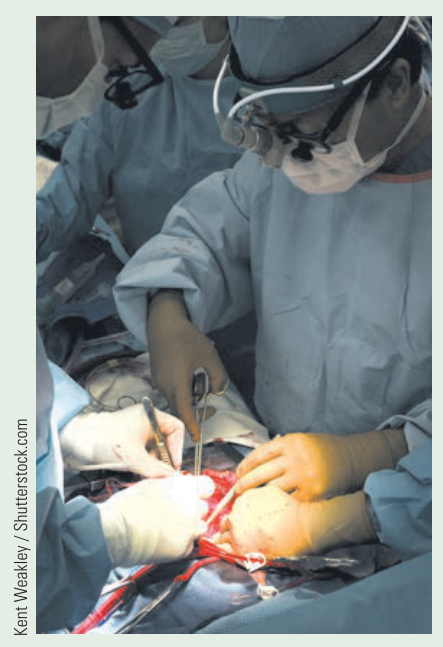
\includegraphics[width=\linewidth]{images/p0282_fig1.png}
    \end{minipage}
  \end{minipage}%
  \hfill
  \begin{minipage}[t]{0.72\textwidth}
    \vspace{0pt}
    \fontsize{8.7pt}{11.5pt}\selectfont
    Thể tích máu điển hình trong cơ thể người là khoảng $5\text{ L}$. Một tỷ lệ phần trăm nhất định của thể tích đó (gọi là \emph{hematocrit}) bao gồm các tế bào hồng cầu (RBCs); thông thường chỉ số hematocrit khoảng $45\%$ ở nam giới. Giả sử một ca phẫu thuật kéo dài 4 giờ và một bệnh nhân nam bị mất $2{,}5\text{ L}$ máu. Trong suốt ca phẫu thuật, thể tích máu của bệnh nhân được duy trì ở mức $5\text{ L}$ nhờ truyền dung dịch muối sinh lý, dung dịch này hòa lẫn nhanh với máu nhưng làm loãng máu khiến chỉ số hematocrit giảm dần theo thời gian.

    \begin{enumerate}[label=\textbf{\arabic*.}, leftmargin=14pt, itemsep=2pt, topsep=2pt]
      \item Giả sử tốc độ mất hồng cầu tỷ lệ thuận với thể tích hồng cầu, hãy xác định thể tích hồng cầu của bệnh nhân khi kết thúc ca phẫu thuật.
      \item Một thủ thuật gọi là \emph{pha loãng máu đẳng thể tích cấp tính} (ANH) đã được phát triển nhằm giảm thiểu sự mất hồng cầu trong phẫu thuật. Trong thủ thuật này, máu được rút ra từ bệnh nhân trước phẫu thuật và được thay thế bằng lượng tương đương dung dịch muối. Việc này làm loãng máu của bệnh nhân, dẫn đến ít hồng cầu bị mất hơn do chảy máu khi phẫu thuật. Lượng máu đã lấy sau đó được truyền lại cho bệnh nhân sau ca mổ. Tuy nhiên, chỉ có thể rút một lượng máu nhất định vì nồng độ hồng cầu không bao giờ được phép giảm xuống dưới $25\%$ trong phẫu thuật. Lượng máu tối đa có thể rút ra theo quy trình ANH đối với ca phẫu thuật được mô tả trong dự án này là bao nhiêu?
      \item Lượng hồng cầu mất đi khi không có quy trình ANH là bao nhiêu? Lượng mất đi là bao nhiêu nếu quy trình được thực hiện với thể tích tính được trong Câu 2?
    \end{enumerate}
  \end{minipage}
\end{tcolorbox}

\vspace{10pt}

%% Section 3.9 Heading
\noindent
\begin{minipage}[c]{0.22\textwidth}
  \begin{tikzpicture}
    \foreach \y in {0pt, 2.5pt, 5pt, 7.5pt, 10pt, 12.5pt, 15pt} {
      \draw[stewartblue!60, thin] (0,\y) -- (3.2,\y);
    }
  \end{tikzpicture}
\end{minipage}%
\hspace{8pt}%
\begin{minipage}[c]{0.74\textwidth}
  {\Huge\bfseries\color{stewartblue}3.9}\quad {\huge\bfseries Tốc độ liên thuộc}
\end{minipage}

\vspace{8pt}

%% Two-column section below heading
\noindent
\begin{minipage}[t]{0.23\textwidth}
  \vspace{115pt}
  \begin{tcolorbox}[
    colback=lightgreenbg!60!gray!15,
    colframe=lightgreenbg!60!gray!15,
    arc=0mm, boxrule=0pt, left=4pt, right=4pt, top=4pt, bottom=4pt
  ]
    \begin{minipage}{14pt}
      \colorbox{pspurple}{\textcolor{white}{\footnotesize\bfseries PS}}
    \end{minipage}%
    \begin{minipage}{\linewidth-16pt}
      \scriptsize\raggedright
      Theo các Nguyên tắc Giải toán được thảo luận sau Chương 1, bước đầu tiên là phải hiểu bài toán. Điều này bao gồm việc đọc kỹ đề bài, xác định rõ điều đã cho, ẩn số cần tìm và đưa vào các ký hiệu phù hợp.
    \end{minipage}
  \end{tcolorbox}
\end{minipage}%
\hfill
\begin{minipage}[t]{0.74\textwidth}
  \fontsize{9.3pt}{12.5pt}\selectfont
  Nếu ta đang bơm không khí vào một quả bóng bay, cả thể tích và bán kính của quả bóng đều tăng và tốc độ tăng của chúng có mối liên hệ với nhau. Tuy nhiên, việc đo đạc trực tiếp tốc độ tăng của thể tích dễ dàng hơn nhiều so với việc đo tốc độ tăng của bán kính.

  Trong một bài toán tốc độ liên thuộc, ý tưởng chính là tính tốc độ thay đổi của một đại lượng theo tốc độ thay đổi của một đại lượng khác (vốn có thể đo đạc dễ dàng hơn). Phương pháp thực hiện là tìm một phương trình liên hệ hai đại lượng đó, sau đó áp dụng Quy tắc chuỗi để lấy đạo hàm cả hai vế theo biến thời gian.

  \vspace{5pt}
  {\bfseries\color{stewartblue}VÍ DỤ 1}\quad Không khí đang được bơm vào một quả bóng hình cầu sao cho thể tích của nó tăng với tốc độ $100\text{ cm}^3/\text{s}$. Bán kính của quả bóng tăng nhanh đến mức nào tại thời điểm đường kính là $50\text{ cm}$?

  \vspace{3pt}
  {\bfseries\color{stewartblue}LỜI GIẢI}\quad Ta bắt đầu bằng việc xác định hai yếu tố:
  \begin{itemize}[leftmargin=35pt, itemsep=1pt, topsep=1pt]
    \item[] \textit{thông tin đã cho:}
    \item[] \hspace{20pt} tốc độ tăng thể tích không khí là $100\text{ cm}^3/\text{s}$
    \item[] \textit{và ẩn số:}
    \item[] \hspace{20pt} tốc độ tăng bán kính khi đường kính bằng $50\text{ cm}$
  \end{itemize}
  Để biểu diễn các đại lượng này dưới dạng toán học, ta đưa vào một số ký hiệu gợi nhớ:
  \begin{itemize}[leftmargin=35pt, itemsep=1pt, topsep=1pt]
    \item[] Gọi $V$ là thể tích của quả bóng và $r$ là bán kính của nó.
  \end{itemize}
\end{minipage}
